%FOR PDFLATEX USE ONLY
\documentclass[a4paper,12pt]{article}

\usepackage{amssymb,amsmath} %math symbols

\usepackage[margin=2cm]{geometry} %paper geometry

\usepackage[utf8]{inputenc} %allows unicode (including russian) source file
\usepackage[russian]{babel} %docment in russian-style
\usepackage[utf8]{inputenc}
\usepackage[unicode]{hyperref} %links inside of the text
\usepackage[pdftex]{graphicx} %includegraphics pictures
\usepackage{cmlgc} %bold text

\usepackage{array} %arrays

\usepackage{wrapfig}
\usepackage{array}
\usepackage{lipsum}
\usepackage{esvect}
\usepackage{hyperref}
\usepackage{xcolor}
\definecolor{linkcolor}{HTML}{799B03} % цвет ссылок
\definecolor{urlcolor}{HTML}{799B03} % цвет гиперссылок
 
\hypersetup{pdfstartview=FitH,  linkcolor=linkcolor,urlcolor=urlcolor, colorlinks=true}
 
\usepackage{subfig}
\usepackage{calc}
\usepackage{pgfplots,tikz,circuitikz}
\usepackage{pgfplotstable}
\usepackage{tkz-euclide}

\usepackage{centernot}
\usepackage{cancel}

\documentclass{article}
\usepackage{amsmath}
\usepackage{mathtext}
\usepackage[T1,T2a]{fontenc}
\usepackage[utf8]{inputenc}
\usepackage[english, bulgarian, russian]{babel}
\usepackage{tikz}
\usepackage{pgfplots}
\usepackage[export]{adjustbox}
\usepackage[left=2cm,right=2cm,
    top=2cm,bottom=2cm,bindingoffset=0cm]{geometry}

\usepackage{csvsimple}

\begin{document}

\begin{center}
  \LARGE{Работа 2.4.1}\\[0.2cm]
  \LARGE{Определение теплоты испарения жидкости}\\[0.2cm]
  \large{Стрижак Даниил}\\[0.2cm]
\end{center}  
  

\section{Аннотация}

В данной работе измеряется давление насыщенного пара жидкости при разной температуре, по полученным данным вычисляется теплота её испарения с помощью уравнения Клапейрона–Клаузиуса.

\section{Теоретические сведения}
Испарением называется переход вещества из жидкого в газообразное состояние. Чтобы испарение проходило без изменения температуры, к жидкости нужно подводить тепло. Количество теплоты, необходимое для изо- термического испарения одного моля жидкости при внешнем давлении, равном упругости ее насыщенных паров, называется \textit{молярной теплотой испарения}. \\
В настоящей работе для определения теплоты испарения применен косвенный метод, основанный на формуле Клапейрона--Клаузиуса

\begin{equation*}
\frac{dP}{dT}=\frac{L}{T(V_2-V_1)}
\end{equation*}

С помощью уравнения Ван-дер-Ваальса можно получить зависимость P(T), с помощью которой определить искомую величину. 

\begin{equation*}
(P+\frac{a}{V^2})(V-b)=RT
\end{equation*}

В таблице ниже приведены все значения параметров различных жидкостей уранения Ван-дер-Ваальса в условиях данного опыта. 

\begin{center}

  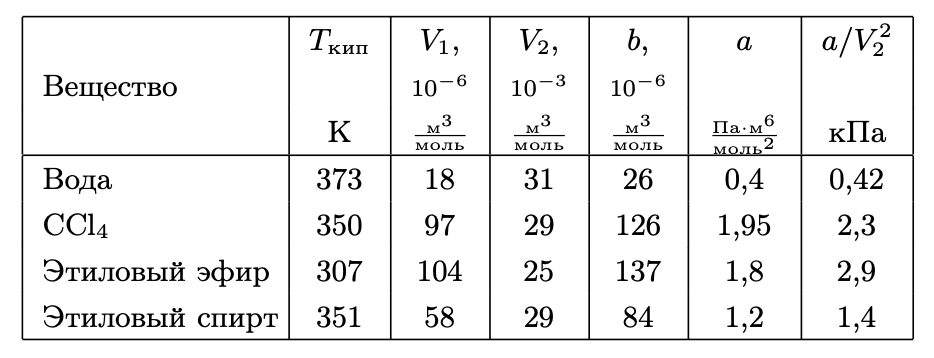
\includegraphics[width=0.7\linewidth]{1.jpg}\\
 
   \\
  
 \end{center}
 
 Откуда видно, что $\frac{V_1}{V_2} < 0.005$, a $\frac{a}{PV^2}<0.03$, ошибка метода измерений равна 4\%, тогда
 
 \begin{equation*}
PV=\nu RT
\end{equation*}
\begin{equation*}
L=\frac{\nu RT^2}{P}\frac{dP}{dT} = -\nu R\frac{lnP}{\frac{1}{T}}
\end{equation*}

\section{Оборудование и инструментальные погрешности}

\textbf{В работе используются:} термостат; герметический сосуд, заполненный исследуемой жидкостью; отсчетный микроскоп.\\
\\textbf{Инструментальные погрешности измерений:}
Градусник -- 0,2 K\\
"Штангенциркуль" -- 0,1 мм\\


\begin{center}
ЭКСПЕРИМЕНТАЛЬНАЯ УСТАНОВКА
\end{center}


\begin{center}
\begin{minipage}{0.47\textwidth}
  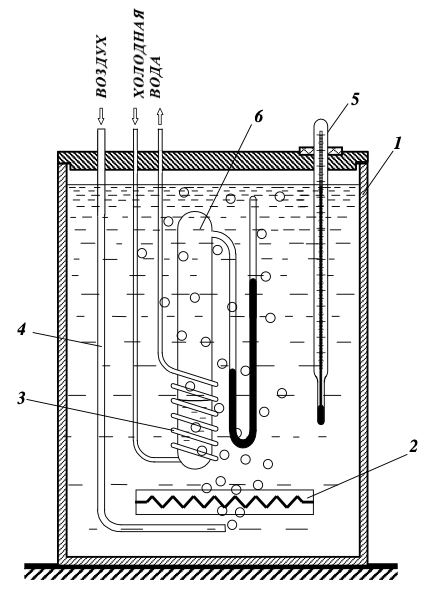
\includegraphics[width=1\linewidth]{2.jpg}
\end{minipage}
\begin{minipage}{0.04\textwidth}
\
\end{minipage}
\begin{minipage}{0.47\textwidth}
 На рисунке слева изображена схема установки.  Наполненный водой резервуар 1 играет роль термостата. Нагревание термостата производится спиралью 2, подогреваемой электрическим током. Для охлаждения воды в термостате через змеевик 3 пропускается водопроводная вода. Вода в термостате перемешивается воздухом, поступающим через трубку 4. Температура воды измеряется термометром 5. В термостат погружен запаянный прибор 6 с исследуемой жидкостью. Над ней находится насыщенный пар (перед заполнением прибора воздух из него был откачан). Давление насыщенного пара определяется по ртутному манометру, соединенному с исследуемым объемом. Отсчет показаний манометра производится при помощи микроскопа.\\
\end{minipage}
\end{center}

\section{Результаты измерений и обработка данных}

\subsection{Подготовка к эксперименту}
Измерим разность уровней в ртутном U - образном манометре с помощью микроскопа и температуру по термометру. Включим термостат. Через каждый градус будем измерять разность высот и температуру. Продолжим повышать температуру в течение половины имеющегося у нас времени, чтобы успеть произвести измерения при остывании прибора. Проведём те же измерения при охлаждении жидкости. Установим такой поток воды, чтобы охлаждение шло примерно тем же темпом, что и нагревание.
\\
\begin{equation*}
P_0 = 1 \ мм. \ рт.\ ст. 
\end{equation*}
\newpage
\subsection{Проведение измерений}
Таблица измерерний при нагревании.
\begin{center}
\begin{tabular}{|c|c|c|c|c|c|c|c|c|c|c|}
\hline
 $  Т,   $ & $    h_1 , $ & $ h_2 ,    $ & $  \Delta h,   $  & $     P,     $ & $  ln(\frac{P}{P_0})         $ & $   1/T,   $ & $    \sigma_P,   $& $   \sigma_{\frac{1}{T}},    $ & $ \sigma_{ln(\frac{P}{P_0})}    ,   $  \\
  $ K   $ & $  мм $ & $  мм    $ & $   мм    $  & $     кПа     $ & $        $ & $    K^{-1} \cdot 10^{-4}   $ & $    \%   $  & $   \%        $& $  \%     $   \\
\hline 
       295,2   &  34        &    80       &    46      &    6,1   &   3,83  &    33,88       &   4,3       &      0,07     &           1,1           \\
\hline 
      296,2    &    33       &   82       &    49      &   6,5    &   3,89  &      33,76     &       4,1   &      0,07     &              1,1        \\
\hline 
        297,2  &     31     &     83      &        52  &     6,9  &   3,95  &    33,65       &     3,8     &       0,07    &             1,0        \\
\hline 
         298,2 &      30    &       84    &      54    &    7,2   &   3,99  &         33,53  &     3,7     &      0,07     &           0,9         \\
\hline 
         299,2 &       28   &      86     &   58       &   7,7    &   4,06  &      33,42     &       3,4   &      0,07     &           0,9           \\
\hline 
         300,2 &      26    &      88     &       62   &  8,3     & 4,13    &       33,31    &      3,2    &     0,07      &           0,8           \\
\hline 
         301,2 &   24       &    90       &     66     &    8,8  &  4,19   &      33,21     &      3,0    &     0,07      &            0,7          \\
\hline
       302,2   &     23     &     92      &    69      &     9,2  &   4,23  &      33,09     &      2,9    &      0,07     &             0,7         \\
\hline 
      303,2    &     20     &     95      &   75      &   10,0    &  4,32   &     32,98      &     2,7     &       0,07    &          0,6            \\
\hline 
     304,2     &    18      &       96    &       78   &     10,4  &   4,36  &     32,87      &     2,6     &       0,07    &            0,6          \\
\hline 
        305,2  &      17    &    97       &   80       &    10,7   &   4,38  &       32,77    &      2,5    &        0,07   &          0,6            \\
\hline 
      306,2    &      14    &     100      &    86      &  11,5     &  4,45   &       32,66    &     2,4     &        0,07   &          0,6            \\
\hline 
        307,2  &      12    &       103    &   91       &   12,1    &    4,51 &     32,55      &     2,2     &       0,07    &        0,5              \\
\hline 
     308,2     &       8   &     105      &     97     &  12,9     &    4,57 &     32,45      &       2,1   &      0,07     &             0,5        \\
\hline 
       309,2   &   6       &     108      &     102     &       13,6&   4,62  &      32,34    &      2,0    &     0,07      &        0,5             \\
\hline
    310,2      &     2     &    112       &      110    &   14,7    &   4,70  &       32,24    &      1,8    &    0,07       &        0,5             \\
\hline 
      311,2    &      1    &     114      &      113    &    15,1   &   4,73  &      32,14     &      1,8    &     0,07      &           0,4          \\
\hline 
     312,2    &     2     &       122    &       120   &     16,0  &   4,79  &    32,03       &     1,7     &      0,07     &          0,4           \\
\hline 
      313,2    &   --       &     --      &      --    &    --   &   --  &    --       &     --     &      --     &    --         \\
\hline 

\end{tabular}

\end{center}
Таблица измерений при охлаждении.

\begin{center}
\begin{tabular}{|c|c|c|c|c|c|c|c|c|c|}
\hline
 $  Т,   $ & $    h_1 , $ & $ h_2 ,    $ & $  \Delta h,   $  & $     P,     $ & $  ln(\frac{P}{P_0})         $ & $   1/T,   $ & $    \sigma_P,   $  &  $   \sigma_{\frac{1}{T}},    $ & $ \sigma_{ln(\frac{P}{P_0})}    ,   $  \\
  $ K   $ & $  мм $ & $  мм    $ & $   мм    $  & $     кПа     $ & $        $ & $    K^{-1} \cdot 10^{-4}   $ & $    \%   $  & $   \%        $ & $  \%       $  \\
\hline 
       295,2   &    32      &    81     &     49   &    6,5   &  3,89   &    33,88       &      4,1    &     0,07      &         1,1            \\
\hline 
      296,2    &     31     &  82      &     51    &     6,8  & 3,93    &      33,76     &     3,9     &      0,07     &           1,0          \\
\hline 
        297,2  &     30     &       84    &     54    &     7,2  &    3,99 &    33,65       &      3,7    &     0,07      &           0,9          \\
\hline 
         298,2 &     28     &       85    &    57      &    7,6   &   4,04  &         33,53  &      3,5    &       0,07    &          0,9            \\
\hline 
         299,2 &    26      & 86          &  60        &   8,0    &  4,09   &      33,42     &      3,3    &      0,07     &          0,9            \\
\hline 
         300,2 &     24     &       89    &     65    &     8,7  &   4,17  &       33,31   &      3,1    &      0,07     &            0,8        \\
\hline
         301,2 &     23     &     90     &    67      &    8,9   &  4,20   &      33,21     &      3,0    &       0,07    &            0,7          \\
\hline 
       302,2   &     22     &      93    &     71     &    9,5   &   4,26  &      33,09     &     2,8     &   0,07        &           0,7           \\
\hline 
      303,2    &      19    &  95     &     76   &    10,1   &  4,33   &     32,98      &      2,6    &      0,07     &            0,6         \\
\hline 
     304,2     &     17     &     98    &     81     &     10,8  &  4,39   &     32,87      &      2,5    &     0,07     &             0,6         \\
\hline 
        305,2  &      15   &  100      &     85     &     11,3  &   4,44  &       32,77    &       2,4   &      0,07     &               0,6       \\
\hline 
      306,2    &      13    &    102       &    89      &    11,9   &  4,49   &       32,66    &    2,2      &      0,07     &           0,5           \\
\hline 
        307,2  &     11    &       104     &      93    &   12,4    &  4,53   &     32,55      &      2,2    &     0,07      &            0,5          \\
\hline 
     308,2     &    8     &    107     &     99     &   13,2    &  4,60   &     32,45      &     2,0     &        0,07   &          0,5           \\
\hline 
       309,2   &      4    &      111    &      107    &   14,3    &  4,67   &       32,34    &     1,9     &    0,07       &               0,4       \\
\hline
    310,2      &     2    &      114     &      112    &   14,9    &  4,72   &       32,24    &     1,8     &        0,07   &             0,4         \\
\hline 
      311,2    &       3   &       120    &      117    &    16,0   &  4,76   &      32,14     &     1,7     &     0,07      &          0,4            \\
\hline 
     312,2    &      1    &       123    &    122     & 16,4      &    4,80 &    32,03       &       1,6   &     0,07      &          0,4            \\
\hline 

\end{tabular}

\end{center}
\subsection{Обработка результатов измерений}


\begin{center}
\begin{tikzpicture}[scale = 2]
\begin{axis}[
    legend style={at={(0.6,0.97)}},
    axis lines = left,
    xlabel = {$T, K$},
    ylabel = {$P, мм.\ рт.\ ст.$},
    xmin=295, xmax=314,
    ymin=40, ymax=125,
	ymajorgrids = true,
	xmajorgrids = true,
	yminorgrids = true, 
	xminorgrids = true, 
	minor tick num = 4 
]
\addplot+[only marks ] plot[error bars/.cd, y dir=both, y explicit]
  coordinates {
	 ( 295.2, 46) 
	 ( 296.2  ,  49)
	 ( 297.2,   52)
	 (  298.2,   54 )
	 (  299.2,  58) 
	 ( 300.2, 62)
	 ( 301.2  ,  66)
	 ( 302.2,   69)
	 (  303.2,   75 )
	 (  304.2,  78)
	 ( 305.2, 80)
	 ( 306.2  ,  86)
	 ( 307.2 ,   91 )
	 (  308.2 ,   97 )
	 (  309.2 ,  102)
	 ( 310.2  ,  110)
	 ( 311.2 ,   113)
	 (  312.2 ,   120 )};

\addplot+[only marks ] plot[error bars/.cd, y dir=both, y explicit]
  coordinates {
	 ( 295.2, 49)
	 ( 296.2  ,  51)
	 ( 297.2,   54)
	 (  298.2,   57 )
	 (  299.2,  60) 
	 ( 300.2, 65)
	 ( 301.2  ,  67)
	 ( 302.2,   71)
	 (  303.2,   76 )
	 (  304.2,  81)
	 ( 305.2, 85)
	 ( 306.2  ,  89)
	 ( 307.2 ,   93 )
	 (  308.2 ,   99 )
	 (  309.2 ,  107)
	 ( 310.2  ,  112)
	 ( 311.2 ,   117)
	 (  312.2 ,   122 )};
	

%\addplot+[brown] coordinates{(  0,0 ) ( 0,0)};	

	
\legend{ 
	$Увеличение\ Т$\\
	$\ \ Уменьшение\ Т\ $\\
	};

\end{axis}
\end{tikzpicture}
\end{center}

Заметно небольшое различие зависимостей давления от температуры при нагревании и охлаждении. \\

Изобразим данные отдельно на двух графиках. Согласно теории необходимо сосчитать производную в каждой точке, для этого воспользуемся методом сплайнов "в первом приближении" (так же будем учитывать строгую монотонность производной в силу итак большой погрешности эксперимента), для чего по каждым трём точкам мысленно построим параболу и найдем её угловой коэффициент. Полученные результаты выпишем в таблицы под графиками. Далее найдём среднее значение теплоты испарения. \\









\newpage
\begin{center}
\begin{minipage}{0.47\textwidth}
\begin{center}
\begin{tikzpicture}[scale = 1]
\begin{axis}[
    legend style={at={(0.4,0.97)}},
    axis lines = left,
    xlabel = {$T, K$},
    ylabel = {$P, мм.\ рт.\ ст.$},
    xmin=295, xmax=314,
    ymin=40, ymax=125,
	ymajorgrids = true,
	xmajorgrids = true,
	yminorgrids = true, 
	xminorgrids = true, 
	minor tick num = 4 
]
\addplot+[only marks ] plot[error bars/.cd, y dir=both, y explicit]
  coordinates {
	 ( 295.2, 46) +- (2,2)
	 ( 296.2  ,  49)+- (2,2)
	 ( 297.2,   52)+- (2,2)
	 (  298.2,   54 )+- (2,2)
	 (  299.2,  58) +- (2,2)
	 ( 300.2, 62)+- (2,2)
	 ( 301.2  ,  66)+- (2,2)
	 ( 302.2,   69)+- (2,2)
	 (  303.2,   75 )+- (2,2)
	 (  304.2,  78)+- (2,2)
	 ( 305.2, 80)+- (2,2)
	 ( 306.2  ,  86)+- (2,2)
	 ( 307.2 ,   91 )+- (2,2)
	 (  308.2 ,   97 )+- (2,2)
	 (  309.2 ,  102)+- (2,2)
	 ( 310.2  ,  110)+- (2,2)
	 ( 311.2 ,   113)+- (2,2)
	 (  312.2 ,   120 )+- (2,2)};
%\addplot[red, domain=3.2:3.4]{0.10952*x^2+8866.44*x-62.208}; 

\end{axis}
\end{tikzpicture}
\end{center}
\end{minipage}
\begin{minipage}{0.47\textwidth}
\begin{center}
\begin{tikzpicture}[scale = 1]
\begin{axis}[
    legend style={at={(0.4,0.97)}},
    axis lines = left,
    xlabel = {$T, K$},
    ylabel = {$P, мм.\ рт.\ ст.$},
    xmin=295, xmax=314,
    ymin=40, ymax=125,
	ymajorgrids = true,
	xmajorgrids = true,
	yminorgrids = true, 
	xminorgrids = true, 
	minor tick num = 4 
]
\addplot+[color=red, fill=red!5, only marks ] plot[error bars/.cd, y dir=both, y explicit]
  coordinates {
	 ( 295.2, 49)+- (2,2)
	 ( 296.2  ,  51)+- (2,2)
	 ( 297.2,   54)+- (2,2)
	 (  298.2,   57 )+- (2,2)
	 (  299.2,  60) +- (2,2)
	 ( 300.2, 65)+- (2,2)
	 ( 301.2  ,  67)+- (2,2)
	 ( 302.2,   71)+- (2,2)
	 (  303.2,   76 )+- (2,2)
	 (  304.2,  81)+- (2,2)
	 ( 305.2, 85)+- (2,2)
	 ( 306.2  ,  89)+- (2,2)
	 ( 307.2 ,   93 )+- (2,2)
	 (  308.2 ,   99 )+- (2,2)
	 (  309.2 ,  107)+- (2,2)
	 ( 310.2  ,  112)+- (2,2)
	 ( 311.2 ,   117)+- (2,2)
	 (  312.2 ,   122 )+- (2,2)};
	
\addplot[red, domain=3.2:3.5]{19.471 - 4.84283 *x}; 
	

%\addplot+[red] coordinates{(   0,0 ) ( 0,0)};
%\addplot+[brown] coordinates{(  0,0 ) ( 0,0)};	

	
%\legend{ 
	%$\ Q = q_{max}$\\
	%$Q = q_1 \ \ \ $\\
	%$Q = q_2 \ \ \ $\\
%};

\end{axis}
\end{tikzpicture}
\end{center}
\end{minipage}
\end{center}

\begin{center}
\begin{minipage}{0.47\textwidth}
\begin{center}

\begin{tabular}{|c|c|c|c|}
\hline
 $  Т,   $ &  $     P,     $  & $  \frac{dP}{dT},   $ & $   L, $  \\
  $ K   $ & $     кПа     $& $    Па/K  $ & $   кДж/кг   $  \\
\hline 
      296,2   &   6,5    & 356 &     847    \\
\hline 
        297,2  & 6,9  &  385 &    891       \\
\hline 
         298,2 & 7,2   &   414  &      854          \\
\hline 
         299,2 &  7,7    &   443  &     854           \\
\hline 
         300,2 &  8,3     & 472    &       852         \\
\hline 
         301,2 &  8,8  &  502   &       868       \\
\hline
       302,2   &  9,2  &   531  &      896       \\
\hline 
      303,2    & 10,0    &  560   &    924           \\
\hline 
     304,2     & 10,4  &   589  &    930          \\
\hline 
        305,2  & 10,7   &   618  &       927        \\
\hline 
      306,2    & 11,5     &  648   &       931      \\
\hline 
        307,2  &  12,1    &    677 &           935            \\
\hline 
     308,2     &  12,9     &   706 &     939        \\
\hline 
       309,2   &  13,6&   735 &      934           \\
\hline
    310,2      &   14,7    &   764  &       904             \\
\hline 
      311,2    &     15,1   &   794  &      920     \\
\hline 

\end{tabular}
\\
Зависимость при увеличении температуры\\
\\
\begin{equation*}
L = 900 \pm  126\frac{кДж}{кг}\ \ \ \varepsilon = 14\%\\
\end{equation*}

\end{center}
\end{minipage}
\begin{minipage}{0.47\textwidth}
\begin{center}

\begin{tabular}{|c|c|c|c|}
\hline
 $  Т,   $ &  $     P,     $  & $  \frac{dP}{dT},   $ & $   L, $  \\
  $ K   $ & $     кПа     $& $    кПа/K  $ & $   кДж/кг   $  \\
\hline 
      296,2   &   6,8  &   363  &      846    \\
\hline 
        297,2  & 7,2  &  392  &   870      \\
\hline 
         298,2 & 7,6   &  421  &         916    \\
\hline 
         299,2 &  8,0    &   451  &      912           \\
\hline 
         300,2 &  8,7     & 480   &       859        \\
\hline 
         301,2 &  8,9  &  509  &      938          \\
\hline
       302,2   &  9,5  &   539  &     936        \\
\hline 
      303,2    & 10,1    &  568 &     904         \\
\hline 
     304,2     & 10,8  &   597 &    925         \\
\hline 
        305,2  & 11,3   &   627 &       933          \\
\hline 
      306,2    & 11,9     &  656   &      934       \\
\hline 
        307,2  &  12,4    &  685 &    842               \\
\hline 
     308,2     &  13,2     &    714 &     841         \\
\hline 
       309,2   &  14,3&   744 &     888           \\
\hline
    310,2      &   14,9    &  773  &    902             \\
\hline 
      311,2    &     16,0   &   802 &     877     \\
\hline 


\end{tabular}
\\
Зависимость при уменьшении температуры\\
\\
\begin{equation*}
L = 892 \pm 131 \frac{кДж}{кг}\ \ \ \varepsilon = 15\%\\
\end{equation*}

\end{center}
\end{minipage}
\end{center}
\begin{equation*}
\frac{\Delta L}{L} = \sqrt{\frac{1}{N^2}\sum\limits_1^n{(4(\frac{\Delta T}{T})^2+(\frac{\Delta P}{P})^2+(\frac{\Delta \frac{dP}{dT}}{\frac{dP}{dT}})^2)}+\frac{1}{N^2}\sum\limits_1^n{(L-\bar{L})^2}+\sigma_{эксп}^2}
\end{equation*}

\newpage
\begin{center}
\begin{minipage}{0.47\textwidth}
\begin{center}
\begin{tikzpicture}[scale = 1]
\begin{axis}[
    legend style={at={(0.4,0.97)}},
    axis lines = left,
    xlabel = {$1/T, K^{-1}$},
    ylabel = {$ln(P/P_0)$},
    xmin=0.003191, xmax=0.00339753,
    ymin=3.78, ymax=4.9,
	ymajorgrids = true,
	xmajorgrids = true,
	yminorgrids = true, 
	xminorgrids = true, 
	minor tick num = 4
]
\addplot+[only marks ] plot[error bars/.cd, y dir=both, y explicit]
  coordinates {
	 ( 0.00338753 , 3.8286)+- (0.043,0.043)
	 ( 0.0033761   ,  3.8918)+- (0.041,0.041)
	 ( 0.00336474  ,   3.9512 )+- (0.038,0.038)
	 (  0.00335345 ,   3.98898 )+- (0.037,0.037)
	 (0.00334225  , 4.0604)+- (0.034,0.034)
	 ( 0.00333111  ,4.1271)+- (0.032,0.032)
 	 (0.00332005   , 4.18965)+- (0.03,0.03)
  (    0.00330907,  4.2341)  +- (0.029,0.029)
   (       0.00329815, 4.317488)   +- (0.027,0.027) 
    (        0.00328731 , 4.3567)    +- (0.026,0.026)
     (             0.00327654 ,4.3820)  +- (0.025,0.025)
      (              0.00326584 ,   4.4543)+- (0.025,0.025)
        (             0.00325521 ,     4.51086)+- (0.024,0.024)
       (               0.00324465 ,     4.5747)+- (0.022,0.022)
         (                 0.00323415 ,  4.62497)+- (0.021,0.021)
          (                  0.00322373 ,4.7)+- (0.02,0.02)
           (                    0.00321337 , 4.7273878)  +- (0.018,0.018)
            (                     0.00320307 ,    4.78749)+- (0.017,0.017)  };



\addplot+[blue] coordinates{(   0,21.25) ( 0.0041345,0)};
%\addplot+[brown] coordinates{(  0,0 ) ( 0,0)};	

	
\legend{ 
	%$\ Q = q_{max}$\\
	%$Q = q_1 \ \ \ $\\
	%$Q = q_2 \ \ \ $\\
};

\end{axis}
\end{tikzpicture}
\\
\\
\ \ \ \ \ \ \ \ \ \ \ \ \ \ \ \ Зависимость при нагревании\\

\ \ \ \ \ \ \ \ \ \ \ \ \ \ \ \ $ \frac{ln(P/P_0)}{1/T} \approx -4980 K$\\

\ \ \ \ \ \ \ \ \ \ \ \ \ \ \ \ L = 898 \pm 81 \frac{кДж}{кг} \ \ \ \ \ \varepsilon = 9\%\\

\end{center}
\end{minipage}
\begin{minipage}{0.47\textwidth}
\begin{center}
\begin{tikzpicture}[scale = 1]
\begin{axis}[
    legend style={at={(0.4,0.97)}},
    axis lines = left,
    xlabel = {$1/T, K^{-1}$},
    ylabel = {$ln(P/P_0)$},
    xmin=0.00319285, xmax=0.00339753,
    ymin=3.8, ymax=4.9,
	ymajorgrids = true,
	xmajorgrids = true,
	yminorgrids = true, 
	xminorgrids = true, 
	minor tick num = 4
]


\addplot+[only marks ] plot[error bars/.cd, y dir=both, y explicit]
  coordinates {
	 ( 0.00338753 , 3.8918)+-(0.041,0.041)
	 ( 0.0033761   ,  3.9318)+-(0.039,0.039)
	 ( 0.00336474  ,   3.98898 )+-(0.037,0.037)
	 (  0.00335345 ,   4.0431 )+-(0.035,0.035)
(0.00334225  , 4.0943)+-(0.033,0.033)
 ( 0.00333111  ,4.1744)+-(0.031,0.031)
 (0.00332005   , 4.2047)+-(0.03,0.03)
  (    0.00330907,  4.2627)  +-(0.028,0.028)
   (       0.00329815, 4.3307)    +-(0.026,0.026)
    (        0.00328731 , 4.3944)    +-(0.025,0.025)
     (             0.00327654 ,4.44265)  +-(0.024,0.024)
      (              0.00326584 ,   4.4886)+-(0.022,0.022)
        (             0.00325521 ,     4.5326)+-(0.022,0.022)
       (               0.00324465 ,     4.59511)+-(0.02,0.02)
         (                 0.00323415 ,  4.6728)+-(0.019,0.019)
          (                  0.00322373 ,4.7184988)+-(0.018,0.018)
           (                    0.00321337 , 4.76217)  +-(0.017,0.017)
            (                     0.00320307 ,    4.8040)+-(0.016,0.016)     };
             
\addplot+[blue] coordinates{(   0,20.5553) ( 0.00418,0)};

	
\legend{ 
	%$\ Q = q_{max}$\\
	%$Q = q_1 \ \ \ $\\
	%$Q = q_2 \ \ \ $\\
};

\end{axis}
\end{tikzpicture}
\\
\\
\ \ \ \ \ \ \ \ \ \ \ \ \ \ \ \  Зависимость при охлаждении\\

\\
\\
\ \ \ \ \ \ \ \ \ \ \ \ \ \ \ \ $\frac{ln(P/P_0)}{1/T} \approx -4920 K$\\
\\
\ \ \ \ \ \ \ \ \ \ \ \ \ \ \ \ L = 888 \pm 79 \frac{кДж}{кг}\ \ \ \ \  \varepsilon = 9\%\\

\end{center}
\end{minipage}
\end{center}

\begin{equation*}
\frac{\Delta L}{L} = \sqrt{\frac{1}{N^2}\sum\limits_1^n{(L-\bar{L})^2}+\sigma_{эксп}^2}
\end{equation*}
 \section{Выводы}
 
Из проделанного эксперимента можно понять, что полученные значения совпадают с табличными с точностью около 5\%, однако, из-за того, что исследуемая жидкость не является чистым спиртом, и в ней скорее всего находится большая массовая доля воды и других спиртов, данная точность удивительна. \\
Заметим, что первый способ обработки гораздо менее точен, чем второй, так как подсчет производных поточечно вносит большую погрешность, сильно влияющую на конечный результат. \\
Так же заметны небольшие различия в значениях разности уровней столбиков при одинаковых температурах при нагревании и охлаждении. Возможно проявляется эффект необратимости термодинамических процессов. Однако данный "гистерезис" не сильно влияет на результат, судя по полученным значениям. \\
Так же в эксперименте  наблюдалось наличие небольшого столбика ртути в одном из колен, его влияние на разность давлений незначительно мало, так как его высота равна приблизительно 2 мм, что в точке с наименьшей разностью столбиков оказывает 3\% ошибку, а с наибольшей -- меньше 1\%. \\
Влияние миниска ртути на разность давлений тоже учитывать не будем, так как измерения проводились от одного края миниска в каждом случае. \\


\end{document}
